\section{Planificación temporal}

La asignación temporal de las tareas que componen este proyecto se puede ver en la Figura \ref{fig:Diagrama de Gantt}. Esta planificación es orientativa y puede sufrir retrasos o modificaciones según avanza el proyecto. Para estimar los costes, se ha considerado una dedicación de 25 horas semanales, con un coste de 22.80€ por hora \cite{Talent.com_2024}.

\subsection{Estimación temporal}

\begin{table}[htbp]
\centering
\begin{tabular}{lcc}
\hline \hline
\textbf{Tarea} & \textbf{Duración (semanas)} & \textbf{Coste} \\
\hline
Revisión bibliográfica & 3 & 1.710,00€ \\
Implementación de modelo híbrido SNN-CNN & 4 & 2.280,00€ \\
Configuración de Framework BindsNET & 0,5 & 285,00€ \\
Optimización de hiperparámetros con Optuna & 1,5 & 855,00€ \\
Selección y preprocesamiento de datos & 2 & 1.140,00€ \\
Experimentación y validación & 3 & 1.710,00€ \\
Análisis comparativo de resultados & 2 & 1.140,00€ \\
Documentación  & 2 & 1.140,00€ \\
\hline
\textbf{TOTAL} & \textbf{18} & \textbf{10.260,00€} \\
\hline \hline
\end{tabular}
\caption{Planificación temporal de tareas, con duración estimada en semanas y coste asociado.}
\label{tab:planificacion_tareas}
\end{table}

Inicialmente nos centraremos en hacer una \textbf{revisión bibliográfica} exhaustiva sobre las redes neuronales de impulsos (SNNs), especialmente su aplicación en detección de anomalías y mantenimiento predictivo. Este análisis nos ayudará a identificar y seleccionar los enfoques y modelos más recientes y relevantes del campo, así como determinar los mejores métodos de optimización multiobjetivo y evaluación comparativa de eficiencia energética entre SNNs y modelos tradicionales.

A continuación, empezaremos con la \textbf{implementación del modelo híbrido SNN-CNN}, añadiendo mejoras como la capa convolucional adaptable y la \textbf{optimización de hiperparámetros mediante frameworks como Optuna}. Prestaremos especial atención a la integración y \textbf{configuración del entorno de trabajo con BindsNET}.

En paralelo vamos a explorar y \textbf{seleccionar las fuentes de datos}, poniendo especial énfasis en la disponibilidad y calidad de conjuntos como IOPS y CalIt2, que necesitan pipelines de preprocesamiento específicos para codificar bien los datos temporales y tratar valores faltantes. Esta etapa es crucial para asegurar que los datos sean adecuados para entrenar y validar bien los modelos de detección de anomalías.

Una vez validada la arquitectura y el procesamiento de datos, lanzaremos la \textbf{fase de experimentación}, implementando escenarios controlados y métricas de evaluación que nos permitan comparar objetivamente el rendimiento y la eficiencia energética frente a modelos tradicionales. \textbf{Los resultados se analizarán} en profundidad, documentando las mejoras arquitecturales y trade-offs identificados, y generando visualizaciones comparativas.

\begin{figure}[p] % [p] = colocar la figura en una página flotante propia
    \centering
    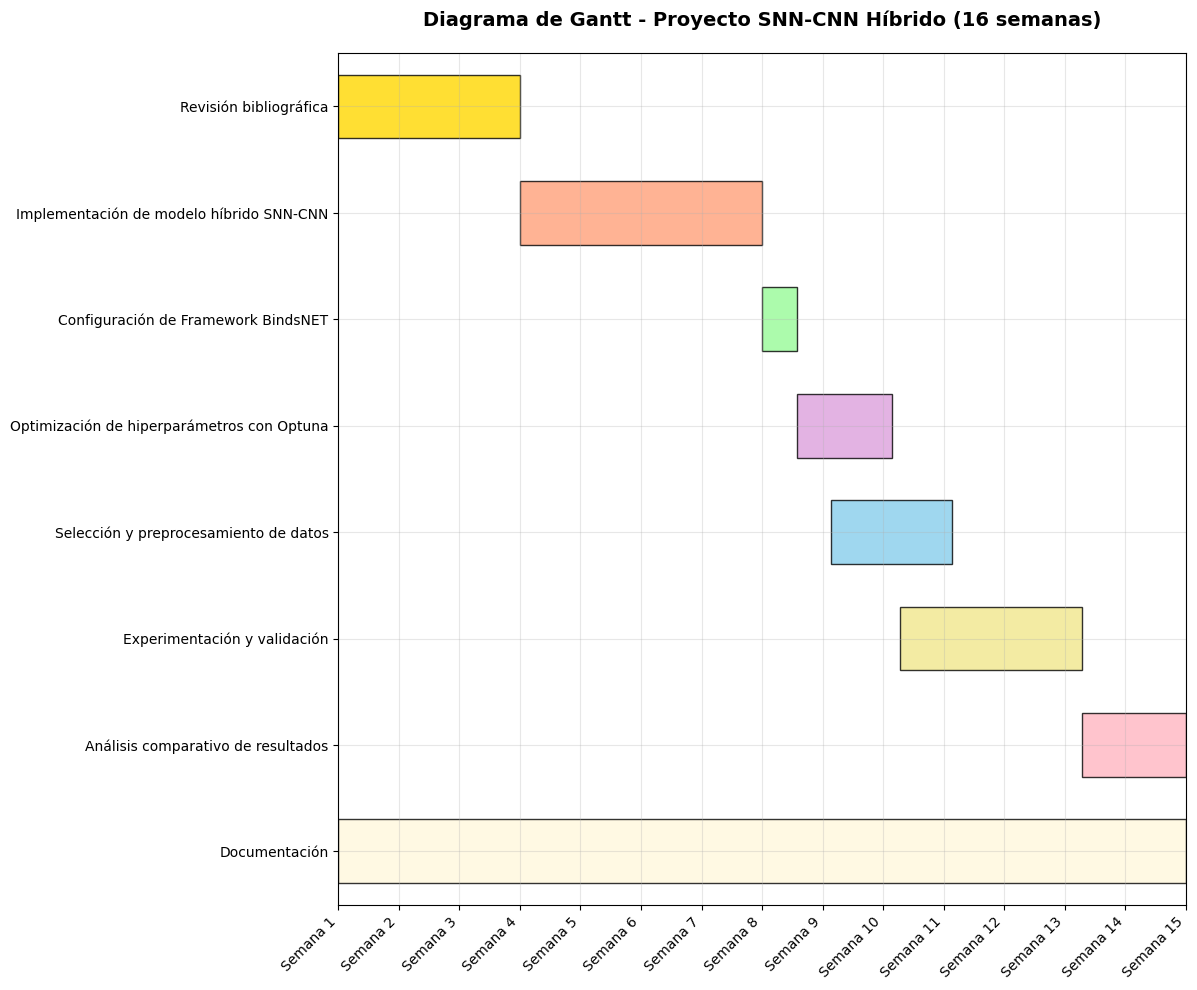
\includegraphics[width=\paperwidth,height=\paperheight,keepaspectratio,angle=90]{Imagenes/Gantt.png}
    \caption{Diagrama de Gantt del proyecto. Fuente: Elaboración propia.}
    \label{fig:Diagrama de Gantt}
\end{figure}